\begin{Example}[marital3]{Marital status and pre- and extramarital sex}
The data on the relation between marital status and reported
premarital and extramarital sex was explored earlier using mosaic
displays in \exref{ex:marital1} and \exref{ex:marital2}.

The $2\times 2 \times 2 \times 2$ table in frequency form can be
analyzed as shown below, where the classification variables are
\pname{GENDER}, \pname{PRE}, \pname{EXTRA}, and \pname{MARITAL}.

\begin{listing}
data marital;
   input gender $ pre $ extra $ @;
    pre = 'Pre:' || pre;
    extra = 'X:' || extra;
   marital='Divorced';  input freq @;  output;
   marital='Married';   input freq @;  output;
datalines;
Women  Yes  Yes   17   4
Women  Yes  No    54  25
Women  No   Yes   36   4
Women  No   No   214 322
Men    Yes  Yes   28  11
Men    Yes  No    60  42
Men    No   Yes   17   4
Men    No   No    68 130
;

proc corresp data=marital mca outc=coords;
    weight freq;
    tables gender pre extra marital;
run;
\end{listing}
The same analysis, with the addition of the 2D plot of
category scores, would be produced by the \macro{CORRESP},
\begin{listing}
%corresp(data=marital, tables=gender pre extra marital, weight=freq, 
   options=mca short, interp=vec, inc=1, pos=-, symbols=dot);
\end{listing}

\begin{Output}[htb]
\caption{Chi-Square Decomposition for Marital status MCA}\label{out:maritalmca1}
\begin{output}
                      Inertia and Chi-Square Decomposition

        Singular  Principal Chi-                                        
        Values    Inertias  Squares Percents    8   16   24   32   40   
                                            ----+----+----+----+----+---
        0.62226   0.38721   1796.45  38.72% ************************    
        0.50915   0.25923   1202.70  25.92% ****************            
        0.43375   0.18814    872.86  18.81% ************                
        0.40672   0.16542    767.47  16.54% **********                  
                  -------   -------                                     
                  1.00000   4639.48 (Degrees of Freedom = 49)           
\end{output}
\end{Output}
%% one figure
\begin{figure}[htb]
  \centering
  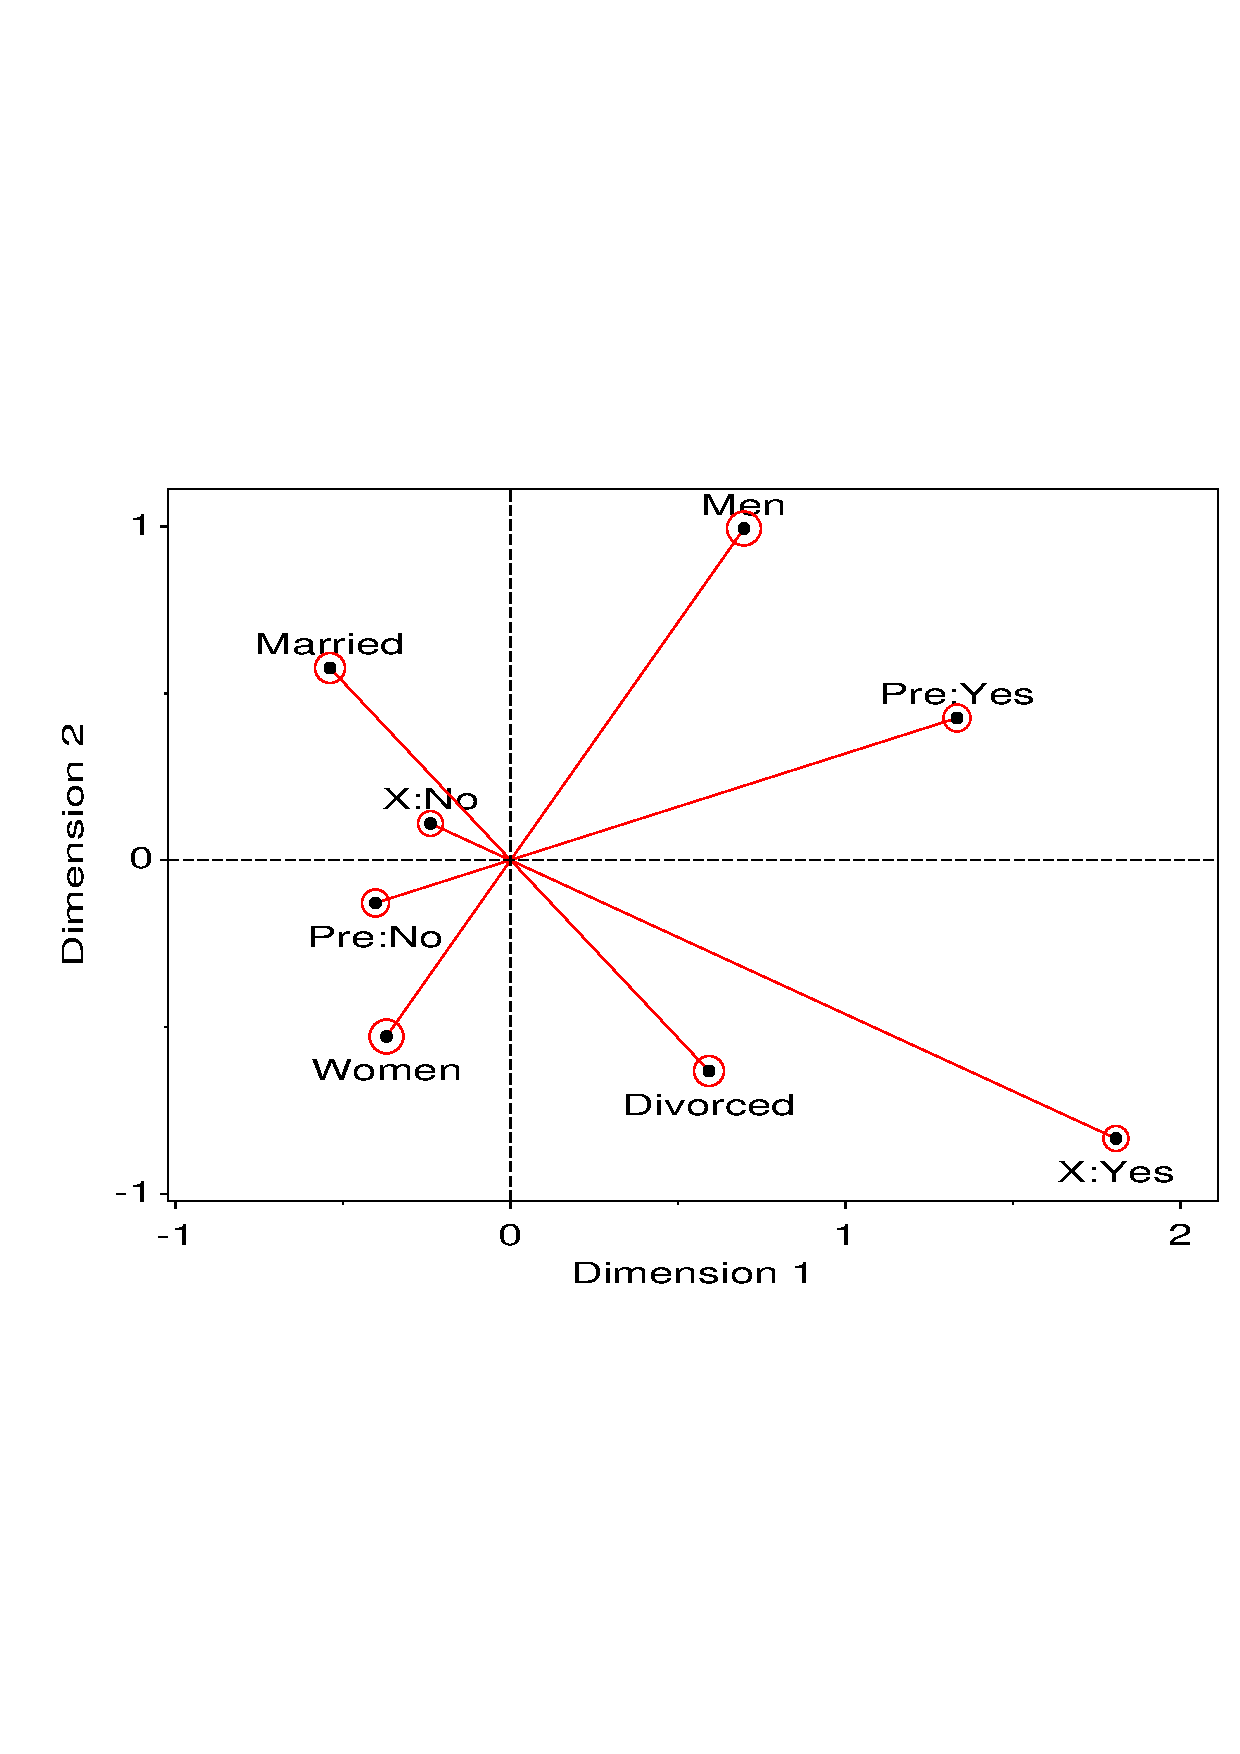
\includegraphics[scale=.8,clip]{ch5/fig/mcamarital1}
  \caption{2D multiple \CA\ display for marital status data}%
  \label{fig:mcamarital1}
\end{figure}

An enhanced version%
\footnote{The size of the bubble symbol surrounding each point is proportional
to the quality of the representation in two dimensions.}
of this plot is shown in \figref{fig:mcamarital1}.
The principal inertias, listed in \outref{out:maritalmca1}, again suggest
that two dimensions are sufficient for this \Dset.
The positions of the category points on Dimension 1 suggest that Women
are less likely to have had pre-marital and extra-marital sex
and that still being married is associated with the absence of pre- and extra-marital sex.

Although two dimensions are probably sufficient for interpreting these
data, we illustrate three-dimensional plots briefly.
When you specify the parameter \pname{DIM=3},
the \macro{CORRESP} produces a coordinates \Dset\ and an \ADS\
with three dimensions.%
\footnote{The first two dimensions are identical to the 2D solution,
because of the nested nature of CA and MCA solutions.}
It also produces a labeled \PROC{G3D} scatter plot.
However, the \pname{G3D} procedure does not allow axes to be equated,
and it is usually necessary to experiment with the \pname{ROTATE}
and \pname{TILT} options to produce a reasonable display, so the plot
generated by the macro should be considered just a first approximation.

A three-dimensional MCA solution for the Marital status data is produced with
this statement:
%% input: /Users/friendly/sasuser/catdata/mcamar.sas
%% last modified: 24-Jul-99 15:56
\begin{listing}
%corresp(data=marital, tables=gender pre extra marital, weight=freq, dim=3, 
   plotreq=dim1 * dim2 = dim3,
   options=mca short, interp=vec, symbols=dot,
   out=coord, anno=label);
\end{listing}
  

To roughly equate the axes,
the initial plot (not shown) was modified by extending the plotting range
for all dimensions as shown below.   Some additional annotation steps
(not shown) produces \figref{fig:mcamarital2}.  Note that the projections
of the points on the Dim1--Dim2 plane is identical to the solution shown
in \figref{fig:mcamarital1}.
%% input: /Users/friendly/sasuser/catdata/mcamar.sas
%% last modified: 21-Jul-99 11:19
\begin{listing}
data xtra;              /* Add dummy points to extend X, Y range */
   input dim1-dim3 shapevar $;
datalines;
 2   1  -.6  POINT
-1  -1  -.6  POINT
data coord;
   Set coord xtra;

goptions vsize=6in hsize=8in;
proc g3d data=coord;
   scatter dim1 * dim2 = dim3
      / shape='point' color='green'
        zmin=-0.6 tilt=80 rotate=75 caxis=gray60
        xticknum=2 yticknum=2 zticknum=2 grid
        annotate=label;
\end{listing}
  
\begin{figure}[htb]
  \centering
  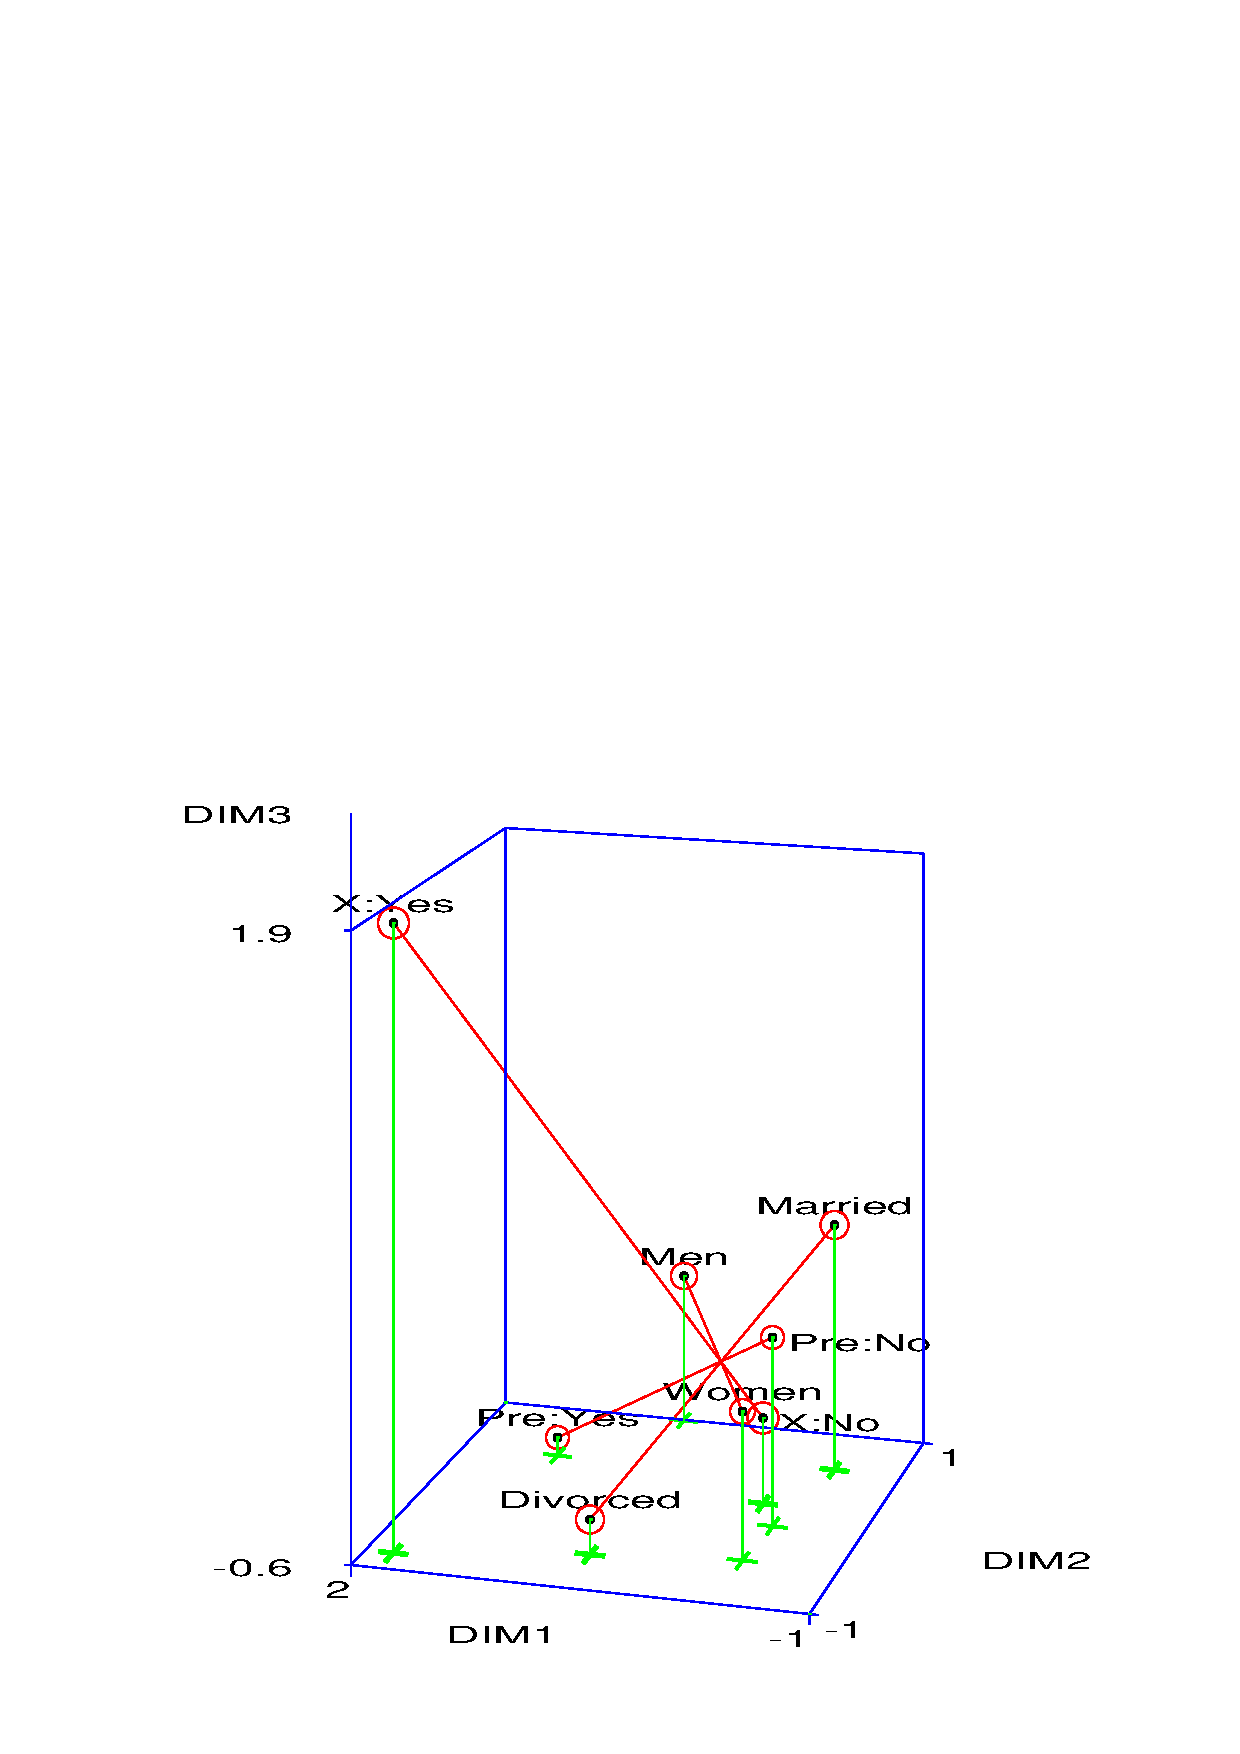
\includegraphics[scale=.8,clip]{ch5/fig/mcamarital2}
  \caption{3D multiple \CA\ display for marital status data}%
  \label{fig:mcamarital2}
\end{figure}
\end{Example}
